\section{Introduction}
\label{sec:intro}

\begin{figure}[t]
  \centering
  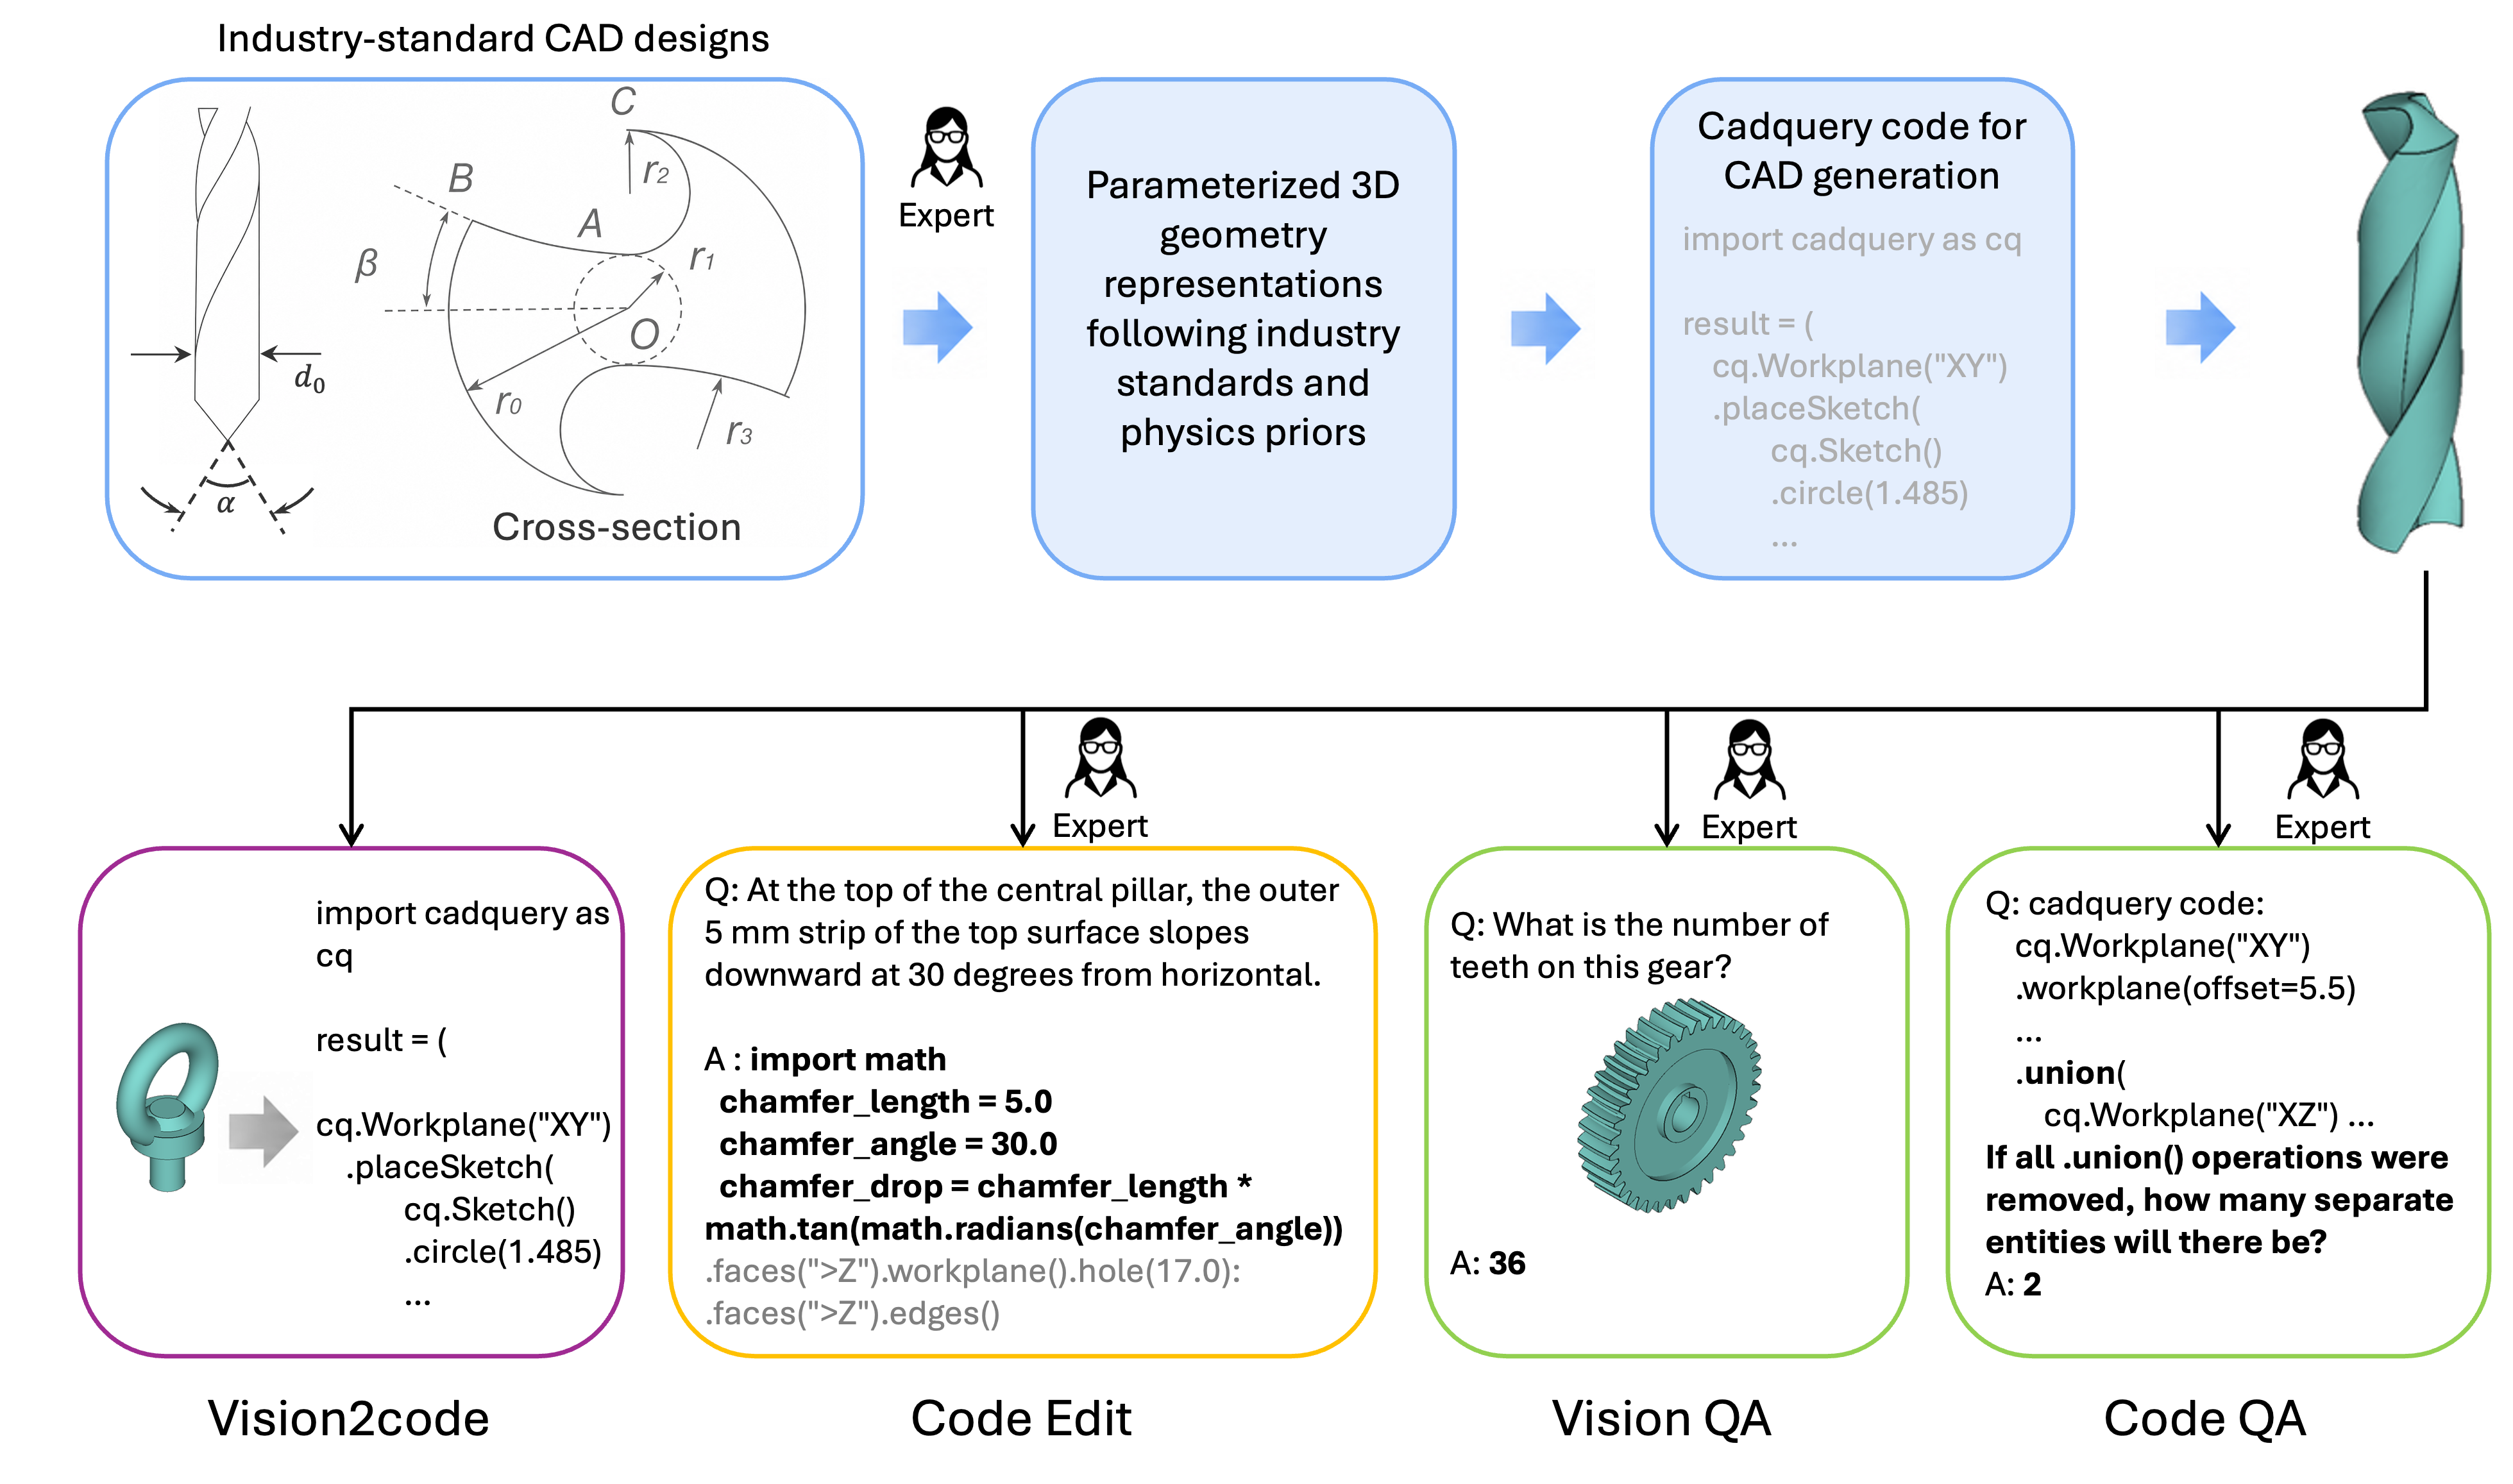
\includegraphics[width=0.78\linewidth]{figures/fig_1.png}
  \caption{\textbf{BenchCAD overview.} \emph{Top:} Parts originate from industry-standard engineering designs (e.g.,\ DIN~338 twist drill cross-section), are realised as parameterised 3D geometry that respects standard parameter relations, and are emitted as executable CadQuery code. \emph{Bottom:} The four BenchCAD evaluation task categories: \texttt{img2cq}, \texttt{edit\_code}, \texttt{qa\_img}, and \texttt{qa\_code}.}
  \label{fig:teaser}
\end{figure}

Large multimodal language models now demonstrate three core capabilities, each individually validated on major benchmarks: \textbf{3D and spatial reasoning from images and code}, \textbf{multi-step CAD operations reasoning}, and \textbf{code generation}.
Programmatic computer-aided design---writing parametric scripts in CadQuery~\citep{CadQuerySoftware} or similar APIs that compile to manufacturable solid geometry---sits at the convergence of all three: producing executable CAD code from an engineering image requires reading geometry, abstracting it into parametric structure, and emitting the precise code.
This convergence makes industrial CAD arguably the next domain where frontier models will land in production. Engineering teams already work in parametric environments, most industrially produced CAD parts are minor variants of a limited set of standard families (gears, fasteners, bearings, springs, brackets, pipes), the dominant workflow involves \emph{editing} an existing parametric program rather than authoring a greenfield design, and the ultimate output is directly manufacturable.
What separates an \emph{industrial} part from a primitive shape is rarely its silhouette---it is the strict compliance with unwritten engineering conventions that every practising designer treats as default (e.g., chamfered grip edges, closed-and-ground spring end coils, involute gear-tooth profiles, fillets at sharp internal corners). These are conventions that no single end-to-end geometry metric directly rewards.
Several recent works have begun to deliver pieces of this promise~\citep{Khan2024,Guan2025,Rukhovich2025,Alrashedy2025,Kolodiazhnyi2026}, yet no public benchmark currently measures, in a systematic and capability-decomposed way, whether today's frontier models clear the stringent bar this domain demands.

A careful look at recent benchmarks reveals an awkward pattern: models that score the highest on Chamfer distance often produce parts that \emph{look} correct in renders but fail every parametric query against the ground truth.
When asked to reconstruct a DIN~338 twist drill (Figure~\ref{fig:teaser}, top) from four canonical views, a state-of-the-art reasoning model emits a CadQuery script whose helix angle, point angle, and flute geometry deviate by 8--22\%, despite the rendered solid passing single-metric IoU evaluation.
\textbf{The geometry passes the eye; it fails the calliper.} The underlying failure mode is structural: a model can recover the outer envelope of an industrial part without ever inferring the parametric structure beneath it, and a single end-to-end metric cannot distinguish the two.
We propose to make this distinction measurable by decomposing the image-to-code pipeline into a three-rung \emph{parametric pyramid} for benchmarking purposes: \textbf{visual + 3D reconstruction} at the base, \textbf{geometric-to-parametric abstraction} in the middle (how a mass-producible standard part maps onto a sequence of CadQuery operations), and \textbf{parametric-to-code synthesis} at the apex.
Prior CAD code-generation benchmarks predominantly reside near the base; the middle rung---the critical step that distinguishes a coarse shape match from an industrially usable parametric program---remains isolated from current public evaluations.

To address this measurement gap, we introduce \textbf{BenchCAD}, a unified, capability-decomposed evaluation framework for large-model CAD reasoning, designed for both today's frontier MLLMs and future CAD agents.
The dataset contains 17{,}900 execution-verified CadQuery parts across 106 industrial part families (49\% anchored to 47 ISO/DIN/EN/ASME/IEC specification codes covering twist drills, bevel gears, compression springs, roller chains, and threaded fittings). These parts exercise 45+ distinct CadQuery operations, including helical sweeps, lofts, twist-extrudes, and parametric involute-gear construction---operation families largely absent from prior corpora.
Atop this dataset, we define four evaluation task categories---\texttt{img2cq} (image-to-code), \texttt{qa\_img}/\texttt{qa\_code} (image- and code-conditioned numeric QA), and \texttt{edit\_img}/\texttt{edit\_code} (instruction-guided editing with verified before/after pairs and a non-target preservation metric). By analyzing score differences across the paired image/code contrasts, we isolate which specific sub-capability bottlenecks a model's performance.

Across 10+ frontier models, we identify three diagnostic phenomena that currently preclude reliable, harnessed CAD design in industry: a \emph{Holistic Spatial and Detailing Deficit}, evidenced by a substantial gap between code- and image-conditioned QA that persists despite chain-of-thought, parameter scaling, and view-count augmentation; an \emph{Industrial Common Sense Gap}, where unwritten engineering conventions are completely absent from the synthesized code; and a \emph{CAD Operational Blindspot}, where matched-compute SFT on sketch+extrude data alone yields zero recall on essential operations until BenchCAD-Synth enters the training mix.
These findings map both the current state of frontier capabilities and the focused improvements required to achieve industry-grade CAD generation.

\paragraph{Contributions.} 
(i) The \textbf{BenchCAD dataset and CadGen pipeline}: 17{,}900 verified parametric CAD parts spanning 106 families (following 47 ISO/DIN/EN/ASME/IEC industrial standard), 2{,}400 paired multi-aspect image and code QA questions covering from basic CAD operations and spatial understanding to parametric reasoning, 748 curated edit pairs, and a 162{,}000-pair training corpus. 
All data and code are released under \texttt{BenchCAD/cad\_bench} on Hugging Face under CC-BY-4.0. 
(ii) A \textbf{unified, capability-decomposed evaluation framework} featuring the first publicly released CAD benchmark that combines execution-verified before/after CadQuery edit pairs with a non-target preservation metric. 
(iii) A \textbf{systematic, capability-decomposed evaluation methodology} that breaks the holistic CAD-generation capability into multiple measurable sub-dimensions and quantifies each independently, rather than collapsing it into a single end-to-end score.
Applied to 10+ frontier vision-language and code-language models, this decomposition surfaces three named diagnostic phenomena---\textbf{Holistic Spatial and Detailing Deficit}, \textbf{Industrial Common Sense Gap}, and \textbf{CAD Operational Blindspot}---refocusing the CAD-LM research agenda toward comprehensive 3D understanding, grounding engineering conventions, and expanding operational coverage in training corpora.